% !TEX encoding = UTF-8 Unicode
\RequirePackage{fix-cm}
\documentclass[a4paper,10pt,UTF8]{paper}
%\documentclass[a4paper,10pt,UTF8]{ctexart}

\usepackage[english]{babel}
\usepackage{fancyhdr,array,lastpage,amsmath,mathtools,enumitem,graphicx,multirow,tocbibind,longtable,makecell,varwidth,titlesec,bm,booktabs,comment,minted,tabularx,multirow,multicol}
\usepackage{enumitem}
\usepackage{hyperref}
\hypersetup{hidelinks}


\usepackage[left=2.54cm,right=2.54cm,top=2.54cm,bottom=2.54cm]{geometry}
\usepackage[font=footnotesize,labelfont=bf]{caption}
\usepackage{tikz,flowchart}
\usepackage{ctex}
\usepackage{xeCJK}%中文字体
\usetikzlibrary{shapes,shapes.geometric,arrows,matrix,calc}
\usetikzlibrary{circuits.logic}

% \usetikzlibrary{circuits.logic.custom}
\usetikzlibrary{circuits.logic.IEC}
\usetikzlibrary{shadows}
\usepackage{listings}
\usepackage[Q=yes]{examplep}
\usepackage{fancyhdr}
\usepackage{alphalph}
\usepackage{indentfirst}

% \setCJKsansfont{黑体}
\setmainfont{PingFang SC}
\setCJKmainfont{PingFang SC}
\setCJKsansfont{PingFang SC}

\usepackage[left=2.54cm,right=2.54cm,top=2.54cm,bottom=2.54cm]{geometry}
\usepackage[font=footnotesize,labelfont=bf]{caption}
\usepackage{tikz,flowchart}
\usepackage{ctex}
\usetikzlibrary{shapes,shapes.geometric,arrows,matrix,calc}
\usetikzlibrary{circuits.logic}
% \usetikzlibrary{circuits.logic.custom}
\usetikzlibrary{circuits.logic.IEC}
\usetikzlibrary{shadows}
\usepackage{listings}
\usepackage[Q=yes]{examplep}
\usepackage{fancyhdr}
\usepackage{alphalph}
\usepackage{indentfirst}

\newenvironment{sol}
  {\par\vspace{2mm}\noindent{\bf Solution}. }

\lstset{escapeinside=``, breaklines=true, frame=none, extendedchars=false, basicstyle=\ttfamily, showstringspaces=false}


\setlength{\parindent}{2em}
\setlength{\parskip}{1.5ex plus 0.5ex minus 0.2ex}
\linespread{1.1}

\bibliographystyle{plain}

\numberwithin{equation}{section}
\numberwithin{figure}{section}

\usepackage{karnaugh}
\usepackage{circuitikz}


\setcounter{secnumdepth}{3}
\setcounter{tocdepth}{3}

\title{华东师范大学计算机科学技术系上机实验报告}

\begin{document}
\pagestyle{fancy}
\chead{\small\color{gray}华东师范大学计算机科学技术系上机实验报告}
\lhead{}
\rhead{}
\makeatletter
\def\headrule{{\if@fancyplain\let\headrulewidth\plainheadrulewidth\fi%
	\color{gray}\hrule\@height 0.2pt\@width\headwidth}
	\vspace{6mm}}
\makeatother

\newcommand{\HRule}{\rule{\linewidth}{1mm}}
\newcommand{\dai}{\textbf{Dais-CMX16$^+$}}

{\center {\huge \bfseries \LARGE{华东师范大学计算机科学技术系上机实验报告}} \\ [0.8cm]
	
	\small{
		\begin{minipage}[t]{.32\linewidth}
			\textbf{课程名称:}计算机组成与结构实践\\
			\textbf{指导教师:}金健\\
			\textbf{上机实践名称:} TODO\\
			\textbf{实践编号:}实验 1
		\end{minipage}
		\begin{minipage}[t]{.32\linewidth}
			\textbf{年级:}17 级\\
			\textbf{姓名:}朱桐\\
			\textbf{学号:}10175102111\\
			\textbf{组号:}A
		\end{minipage} 
		\begin{minipage}[t]{.32\linewidth}
			\textbf{上机实践成绩:} \\
			\textbf{创新实践成绩:} \\
			\textbf{上机实践日期:}2019/09/20\\
			\textbf{上机实践时间:}2 学时\\
		\end{minipage}
	}
	\HRule \\[0.5cm]
}
\section{实验目的}

\begin{enumerate}
	\item 掌握微指令的编码结构和编码方法
	\item 掌握微程序的执行方式(宏观和微观)
	\item 掌握机器指令与微程序的关系
\end{enumerate}

\section{实验设备}

\dai 一台

\section{实验内容}

\begin{enumerate}
	\item 指令微地址的形成实验
	\item 后续微地址的形成实验
\end{enumerate}


\section{实验原理}

\subsection{控制器组成}

控制器是计算机的指挥和控制中心,由它把计算机的运算器、存储器、I/O 设备等联系成一个有机的系统,并根据程序所特定的微指令序列对各部件的具体要求,适时地发出各种命令,控制计算机各部件有条不紊的进行工作。

如图 \ref{fig:1} 所示,本系统控制器由组合逻辑与存储逻辑集合组成。两者按独立控制器的规范与标准设计,既可单独控制,亦可交替互补(混合)控制,在国内率先把 PLA 控制理念融入微控制器的设计与实现中。

\begin{figure}[h]
	\centering
	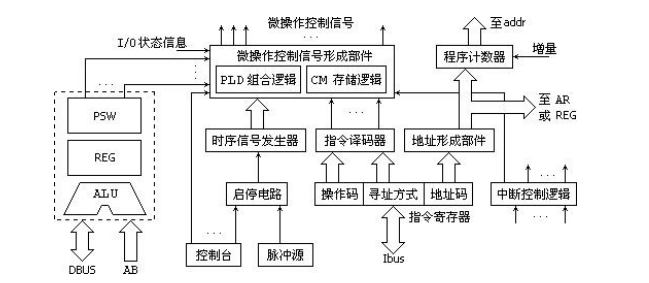
\includegraphics[width=0.9\textwidth]{1.PNG}
	\caption{控制器组成框图}
	\label{fig:1}
\end{figure}

\subsubsection{组合逻辑型}

如图 \ref{fig:1} 所示的 PLD 框为组合逻辑型控制器,由可编程器件 XC9572 独立组成,在器件编程环境的支撑下完成微操作控制信号的设计与下载。以取得最高操作速度为设计目标,它的缺点是繁锁、杂乱、缺乏规律性,且不易修改和扩充,缺乏灵活性。

组合逻辑控制器实质上是一个组合逻辑电骆,它将一组输入逻辑信号转換成一组输出控制信号,可称为硬布线控制器。

\subsubsection{存在逻辑型}

如图 \ref{fig:1} 所示的 CM 框为存储逻辑型微程序控制器,它是采用存储逻辑来实现的,也就
是把微操作信号代码化,使每条机器指令转化成为一段微程序,存入控制存储器中,微操作控制
信号由微指令产生。

微程序控制器的设计思想和组合逻辑的设计思想截然不同。它具有设计规整,调试、维修以
及更改、扩充指令方便的优点,易于实现自动化设计,已成为当前控制器的主流。但是,由于它
增加了一级控制存储器,所以指令的执行速度比组合逻辑控制器慢。

\subsubsection{组合逻辑与存储逻辑结合}

如图 \ref{fig:1} 所示,本系统控制器由组合逻辑与存储逻辑集合组成 PLA 控制器,它是吸收前
两种的设计思想来实现的。PLA 控制器实际上也是一种组合逻辑控制器,但它又与常规的组合
逻辑控制器的硬联结构不同,它是程序可编的,某一微操作控制信号由存储逻辑控制器产生。

\subsubsection{关于组合逻辑控制器实验}

组合逻辑控制器由大规模可编程器件的软逻辑设计定义,渉及器件的开发环境,我们在基于
“RISC”处理器构成的模型机实验中论证。这里以微程序控制器为例展开控制器的原理组成与
顺序控制实验。

\subsection{微程序控制器}

微程序控制的实质是用程序设计的思想方法耒组织微操作控制逻辑,用规整的存储逻辑代替
繁杂的组合逻辑。把各条指令的微操作序列以二进制编码字的形式设计成微程序,存放在控制存
储器中,通过读取并执行相应的微程序实现一条指令的功能。这就是微程序控制的基本概念。



\subsubsection{微程序控制器的组成结构}

\begin{figure}[h]
	\centering
	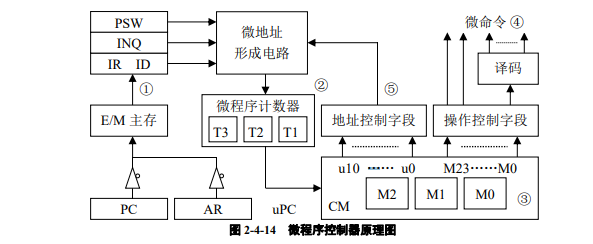
\includegraphics[width=0.9\textwidth]{2.PNG}
	\caption{微程序控制器原理图}
	\label{fig:2}
\end{figure}

1) 控制存储器 CM

如图 \ref{fig:2} 所示的 CM 框为微程序控制器,由 2 片 6264 和 1 片 6116 共三片静态存储器平
行组成。它们的地址通路由微程序计数器PC 供给,其寻址范围为 0~7FF.控制器设有段微址,2
片 6264 的数据端在段微址的指示下分时输出下址与微控制信息,并和 6116 的数据端平行组成
24 个途经三态门隔离驱动的微控制位(M23~M0)。

2)微程序计数器$\mu PC$

图 \ref{fig:2} 所示的微地址计数器框由 3 片 161 构成按字方式寻址的PC 计数器,计数器的输
入端通过微总线($\mu BUS$)从指令译码器 ID、微控制器(CM)的下址段捕捉非因变分量,从运
算标志 PSW、中断请求标志 INQ 等标志中捕捉因变分量。计数器的输出端组成 12 位微地址总
线,控制微程序存储器的寻址。其中 ua11 为段微址,电路构造中与 2 片 6264 的地址端“A11”
相连,它零状态输出微控制信息,“1”状态输出下续微地址。它的清零端由中央外理器单元直控,
上电时 $\mu PC$ 计数器自动淸零,实验中按【返回】键亦可实现计数器的手动淸零。

\subsection{微程序的执行过程}

图 2-4-14 所标示的字号表示微程序控制的全部工作过程。

\begin{enumerate}
	\item 启动取指微指令或微程序,根据程序计数器 PC 所提供的指令地址,从 EM 主存中取出所要执行的机器指令,送入指令寄存器 IR、指令译码器 ID 中,并且完成 PC+1,指向机器指令的下址单元。
	\item 根据 ID 译码器中的指令码,把微地址形成电路产生的机器指令起始微地址打入 $\mu PC$
	\item 从PC 所指定的 CM 控制存储器单元分时输出微操作控制字段与下续微地址控制字段。
	\item 微指令的操作控制字段经译码或直接产生一组微命令,控制有关功能部件完成微程序所规定的微操作。
	\item )微指令的下址段及当前 PSW、INQ 等标志送往微地址形成电路,产生下条微指令的地址,进入读取与执行下条微指令。如此循环,直到一条机器指令的微程序全部执行完毕。
\end{enumerate}

\subsection{微指令格式及编码}

\begin{figure}[h]
	\centering
	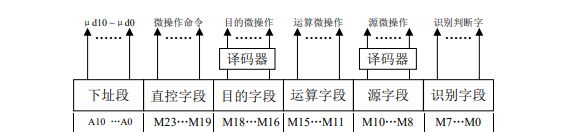
\includegraphics[width=0.9\textwidth]{3.PNG}
	\caption{微指令控制格式}
	\label{fig:3}
\end{figure}


本系统采用字段直接编码法,把微指令操作控制字段划分为若干个子字段,每个子字段的所有微命令进行统一编码。

如图 \ref{fig:3} 所示,本控制器微指令字长 35 位,其中 24 个操作控制位分别由识别判断字段、
运算控制字段、源寻址字段、目的寻址字段及直接控制字段组成。在下址捕捉时段由 M18~M8
输出字为 11 位的后续微地址。

\subsubsection{识别字段}

M4、M1、M0 分别定义 Iμ、Icz、Ids,组成下址识别字段。它们的编码下表所示。
\section{实验步骤}

\section{调试过程、结果与分析}

\section{总结}

\section{附件}

\end{document}
